% =====================================================================
% Guía del estudiante -- Física 10° -- Trimestre I
% Hilo conductor: De la inercia a los Principia
% Temas (propuesta de curriculo/plan-anual.md, clases 005-022):
%   medicion, vectores, cinematica, primeraley, segundaley, terceraley, tresleyes
% Plan: guia-periodo-I-leyes-newton.plan.md
% =====================================================================
% Plan del trimestre aprobado por la docente el 2026-09-18. Esta guía es todavía el borrador de
% la generación rápida del 2026-09-14: falta rehacerla con el proceso de tres etapas.
\documentclass[11pt]{article}
\makeatletter\def\input@path{{../../../../plantillas/estilo/}}\makeatother
\usepackage{mmcantillo}

% ======================== DATOS DE LA GUÍA ============================
\tipodocumento{Guía del estudiante}
\asignatura{Física}
\titulo{Fuerza y movimiento: las leyes de Newton}
\grado{10°}
\periodo{I}
\hiloconductor{De la inercia a los \emph{Principia}}
% ======================================================================
% DBA: naturales grado 10 · DBA 1 — Comprende, que el reposo o el movimiento rectilíneo
% uniforme, se presentan cuando las fuerzas aplicadas sobre el sistema se anulan entre ellas,
% y que en presencia de fuerzas resultantes no nulas se producen cambios de velocidad.
% (dba/naturales/grados/grado10.tex; el tema de medición no tiene DBA: es herramienta.)

\begin{document}

\encabezado

% ---------------------------------------------------------------------
% 1. Frase introductoria
% ---------------------------------------------------------------------
% verificado: https://digitallibrary.hsp.org/index.php/detail/objects/9792 — original: «If I have seen further it is by standing on ye sholders of Giants» (Historical Society of Pennsylvania)
\frase{Si he visto más lejos es porque estoy de pie sobre hombros de gigantes.}
{Isaac Newton, carta a Robert Hooke (5 de febrero de 1675/76)}

% ---------------------------------------------------------------------
% 2. Introducción
% ---------------------------------------------------------------------
\seccion{Introducción}

¿Por qué te vas hacia adelante cuando el bus frena de golpe? ¿Por qué cuesta más empujar un
carro que una bicicleta? ¿Qué empuja a un cohete en el espacio vacío? En noveno aprendiste a
\emph{describir} el movimiento; en este trimestre vamos a \emph{explicarlo}: a encontrar sus
causas, las fuerzas, y las tres leyes que las relacionan con los cambios de velocidad.

Nuestro hilo conductor va de un plano inclinado en Italia a un libro publicado en Londres en
1687. Galileo imaginó un mundo sin roce y descubrió la inercia; Isaac Newton, apoyado en él y
en otros «gigantes», escribió las tres leyes del movimiento en los \emph{Principia}; y
Émilie du Châtelet tradujo y comentó esa obra para que media Europa pudiera leerla. En cada
tema daremos un paso de esa historia.

\textbf{Al terminar este trimestre podrás:}
\begin{itemize}
  \item expresar medidas en unidades del SI, con notación científica y cifras significativas;
  \item sumar vectores ---desplazamientos y fuerzas--- de forma gráfica y por componentes;
  \item predecir si un cuerpo está en equilibrio a partir de su diagrama de cuerpo libre;
  \item calcular la aceleración de un cuerpo a partir de la fuerza neta y su masa;
  \item identificar pares de acción y reacción, de contacto y a distancia.
\end{itemize}

Este trimestre trabaja el siguiente Derecho Básico de Aprendizaje del Ministerio de Educación
Nacional~\cite{mendba}. El primer tema (medición) no corresponde a ningún DBA: es una
herramienta que usaremos todo el año.

\begin{dba}[Grado 10 · DBA 1]
Comprende, que el reposo o el movimiento rectilíneo uniforme, se presentan cuando las fuerzas
aplicadas sobre el sistema se anulan entre ellas, y que en presencia de fuerzas resultantes no
nulas se producen cambios de velocidad.
\end{dba}

% ---------------------------------------------------------------------
% 3. Marco teórico
% ---------------------------------------------------------------------
\seccion{Marco teórico}

\subsubsection*{Galileo y la inercia}

Para Aristóteles, un cuerpo se detiene si nada lo empuja. Galileo (1564--1642) no estuvo de
acuerdo. Observó que un objeto liso se desliza sobre una mesa más lejos que uno áspero, y uno
todavía más liso, más lejos aún; e imaginó el caso límite, un plano sin ningún roce: allí un
cuerpo en movimiento seguiría moviéndose con rapidez constante en línea recta, sin que nada
lo empujara~\cite{recurso10}. En sus \emph{Discursos} de 1638 estudió además la caída con
esferas que rodaban por un canal inclinado y un reloj de agua~\cite{galileo1638}. (La historia
de las bolas lanzadas desde la torre de Pisa no está documentada: viene de una biografía
escrita por su secretario Vincenzo Viviani en 1654 y los historiadores la consideran una
leyenda~\cite{physicsworld}.)

\subsubsection*{Halley, Newton y un libro de 1687}

En 1684 el astrónomo Edmond Halley visitó a Isaac Newton en Cambridge para preguntarle por la
forma de las órbitas de los planetas, y descubrió que Newton ya tenía la respuesta pero no la
había publicado. Halley lo animó a escribirla, corrigió las pruebas de imprenta y, como la
Royal Society no tenía dinero en ese momento, pagó la edición de su bolsillo~\cite{halley}. Así
se publicaron en Londres, en 1687, los \emph{Philosophiæ Naturalis Principia Mathematica}
(«Principios matemáticos de la filosofía natural»)~\cite{newton1687}. Al comienzo del libro,
Newton enuncia sus tres leyes del movimiento:

% verificado: https://www.thelatinlibrary.com/newton.leges.html — Principia, 3.ª ed. (1726): «Lex I. Corpus omne perseverare in statu suo quiescendi vel movendi uniformiter in directum, nisi quatenus illud a viribus impressis cogitur statum suum mutare. Lex II. Mutationem motus proportionalem esse vi motrici impressæ, & fieri secundum lineam rectam qua vis illa imprimitur. Lex III. Actioni contrariam semper & æqualem esse reactionem: sive corporum duorum actiones in se mutuo semper esse æquales & in partes contrarias dirigi.»
\begin{cita}{Isaac Newton, \emph{Principia}, «Axiomas o leyes del movimiento» (3.ª ed., 1726), trad. propia del latín~\cite{newton1726}}
Ley I. Todo cuerpo persevera en su estado de reposo o de movimiento uniforme en línea recta, a
menos que sea obligado a cambiar ese estado por fuerzas impresas sobre él.

Ley II. El cambio de movimiento es proporcional a la fuerza motriz impresa y se produce según
la línea recta en que esa fuerza se imprime.

Ley III. A toda acción se opone siempre una reacción igual; es decir, las acciones mutuas de
dos cuerpos son siempre iguales y dirigidas en sentidos contrarios.
\end{cita}

¿Y la manzana? En abril de 1726, ya anciano, Newton le contó a su amigo William Stukeley que
la idea de la gravitación le había venido al ver caer una manzana en el jardín de su casa
familiar; Stukeley lo escribió en sus memorias de 1752~\cite{stukeley}. Es una anécdota
contada por el propio Newton sesenta años después de los hechos: bonita, pero no un dato
comprobado.

\subsubsection*{Émilie du Châtelet: los \emph{Principia} en francés}

Los \emph{Principia} estaban en latín y eran dificilísimos. Émilie du Châtelet (1706--1749),
matemática y filósofa natural francesa, había publicado en 1740 sus \emph{Instituciones de
física}, y dedicó sus últimos años a traducir los \emph{Principia} al francés con un
comentario propio en el que añadió cálculos y resultados posteriores a Newton. Terminó el
trabajo poco antes de morir, en 1749; se publicó en 1756 y completo en 1759, y todavía hoy es
la traducción francesa de referencia~\cite{sepChatelet,chatelet1759}.

\subsubsection*{Medir hoy}

Newton y Galileo medían con relojes de agua y patrones que variaban de ciudad en ciudad. Hoy
el Sistema Internacional define sus unidades a partir de constantes de la naturaleza: desde el
20 de mayo de 2019, por ejemplo, el kilogramo se define fijando el valor de la constante de
Planck~\cite{bipm}.

% ---------------------------------------------------------------------
% 4. Temas
% ---------------------------------------------------------------------
\tema{Medición}\label{tema:medicion}

\begin{hilo}
Galileo medía el tiempo pesando agua. Antes de estudiar fuerzas, necesitamos lo mismo que él:
medir bien, en unidades que todos entiendan, y saber cuánto confiar en cada número.
\end{hilo}

Las magnitudes \textbf{fundamentales} del SI que usaremos son la longitud (metro, m), la masa
(kilogramo, kg) y el tiempo (segundo, s); las demás, como la velocidad (m/s) o la fuerza
(newton, N), son \textbf{derivadas}. Los prefijos son potencias de diez: kilo ($10^3$), centi
($10^{-2}$), mili ($10^{-3}$), micro ($10^{-6}$), nano ($10^{-9}$). En \textbf{notación
científica} un número se escribe $a \times 10^{n}$ con $1 \le |a| < 10$; por ejemplo,
$\qty{0,000045}{m} = \qty{4,5e-5}{m}$. Y para convertir unidades se multiplica por factores
iguales a uno:
\[
  72\,\frac{\text{km}}{\text{h}} \cdot \frac{1000\ \text{m}}{1\ \text{km}} \cdot
  \frac{1\ \text{h}}{3600\ \text{s}} = \qty{20}{m/s}.
\]

Toda medida tiene incertidumbre. Las \textbf{cifras significativas} son las que se conocen con
confianza: en una multiplicación o división, el resultado lleva tantas como el dato que menos
tenga; en una suma o resta, tantos decimales como el dato menos preciso~\cite{recurso10}.

\begin{ejemplo}[El área de una tarjeta]
Una tarjeta mide \qty{4,5}{cm} por \qty{3,25}{cm}. La calculadora da $\num{14,625}$, pero
\qty{4,5}{cm} solo tiene dos cifras significativas: el área es \qty{15}{cm^2}.
\end{ejemplo}

\begin{aplicacion}[El orden de magnitud como alarma]
Antes de calcular, un físico estima. Si una conversión te dice que un carro va a
\qty{324}{m/s}, casi la rapidez del sonido, sabes que algo salió mal antes de revisar la
cuenta. Estimar el orden de magnitud no reemplaza el cálculo: lo protege.
\end{aplicacion}

\begin{preguntas}
% Ejercicio: mediciones-10-001
\pregunta El área de un rectángulo de $\num{4,5}$ cm por $\num{3,25}$ cm se da correctamente
con:
\begin{opciones*}(4)
  \item $\num{14,625}\ \mathrm{cm^2}$
  \item $\num{14,63}\ \mathrm{cm^2}$
  \item $\num{14,6}\ \mathrm{cm^2}$
  \item $15\ \mathrm{cm^2}$
\end{opciones*}
% Ejercicio: mediciones-10-058
\pregunta Expresa la siguiente suma con el número correcto de cifras significativas:
$\num{1,80}\ \text{m} + \num{142,5}\ \text{cm} + \num{5,34e5}\ \mu\text{m}$.
\espacio{2.5cm}
% Ejercicio: mediciones-10-055
\pregunta Si un avión viaja a $950$ km/h, ¿cuánto tiempo le tomará recorrer $\num{1,00}$ km?
\espacio{2cm}
% Ejercicio: mediciones-10-062
\pregunta Estima el orden de magnitud (potencia de diez) de $2800$.
\espacio{1cm}
\end{preguntas}

\begin{resumen}
\begin{itemize}
  \item Unidades fundamentales: m, kg, s. Los prefijos son potencias de diez.
  \item Se convierte multiplicando por factores iguales a uno.
  \item En productos y cocientes manda el dato con menos cifras significativas; en sumas, el
        de menos decimales.
  \item Estimar el orden de magnitud sirve para detectar errores.
\end{itemize}
\end{resumen}

% ---------------------------------------------------------------------
\tema{Vectores}\label{tema:vectores}

\begin{hilo}
Newton habla de fuerzas «impresas» que tienen una dirección: la segunda ley dice que el cambio
de movimiento ocurre «según la línea recta» en que actúa la fuerza. Para trabajar con sus
leyes necesitamos cantidades con dirección: los vectores.
\end{hilo}

Una magnitud \textbf{escalar} queda definida con un número y una unidad (masa, tiempo,
temperatura). Una magnitud \textbf{vectorial} necesita además dirección y sentido
(desplazamiento, velocidad, fuerza). Dos vectores se suman gráficamente poniendo el origen del
segundo en la punta del primero. Para calcular, se descompone cada vector en
\textbf{componentes}: un vector de magnitud $V$ que forma un ángulo $\theta$ con el eje $x$
tiene $V_x = V\cos\theta$ y $V_y = V\operatorname{sen}\theta$. Se suman las componentes y se
recupera la resultante con
\[
  R = \sqrt{R_x^2 + R_y^2}, \qquad \tg\theta = \frac{R_y}{R_x}.
\]

\begin{ejemplo}[Dos fuerzas perpendiculares]
Sobre una caja actúan \qty{30}{N} hacia el oriente y \qty{40}{N} hacia el norte. La fuerza
neta es $\sqrt{30^2 + 40^2} = \qty{50}{N}$, en la dirección $\theta = \arctg(40/30) \approx
\ang{53,1}$ al norte del oriente.
\begin{center}
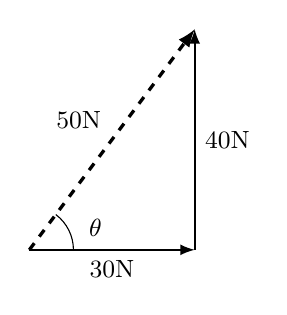
\begin{tikzpicture}[>=latex, scale=0.07, font=\small]
  \draw[->, thick] (0,0) -- (30,0) node[midway, below] {\qty{30}{N}};
  \draw[->, thick] (30,0) -- (30,40) node[midway, right] {\qty{40}{N}};
  \draw[->, very thick, dashed] (0,0) -- (30,40) node[midway, above left] {\qty{50}{N}};
  \draw (8,0) arc (0:53.1:8); \node at (12,4) {$\theta$};
\end{tikzpicture}
\end{center}
\end{ejemplo}

\begin{aplicacion}[El GPS y los vectores]
Una aplicación de navegación registra cada tramo de tu recorrido como un vector (cuánto y
hacia dónde) y los suma por componentes para saber dónde estás respecto al punto de partida.
\end{aplicacion}

\begin{preguntas}
% Ejercicio: cinematica-2d-10-007
\pregunta Dos vectores tienen magnitudes $V_1 = \num{3,5}$ km y $V_2 = \num{4,0}$ km. ¿Cuáles son
las magnitudes máxima y mínima de su suma vectorial?
\espacio{2cm}
% Ejercicio: cinematica-2d-10-031
\pregunta Si $V_x = \num{7,80}$ unidades y $V_y = -\num{6,40}$ unidades, determina la magnitud
y la dirección de $\vec V$.
\espacio{2.5cm}
% Ejercicio: cinematica-2d-10-030
\pregunta Un camión repartidor recorre 28 cuadras al norte, 16 al este y 26 al sur. ¿Cuál es
su desplazamiento desde el origen? Las cuadras tienen igual longitud.
\espacio{3cm}
% Ejercicio: cinematica-2d-10-029
\pregunta Un automóvil recorre 225 km al oeste y luego 78 km al suroeste ($45^\circ$). ¿Cuál es
su desplazamiento desde el punto de partida (magnitud y dirección)? Dibuja un diagrama.
\espacio{3.5cm}
% Ejercicio: leyes-newton-10-056
\pregunta Una fuerza de 650 N actúa hacia el noroeste. ¿En qué dirección debe actuar una
segunda fuerza de 650 N para que la resultante apunte hacia el oeste? Ilustra con un diagrama
de vectores.
\espacio{3.5cm}
\end{preguntas}

\begin{resumen}
\begin{itemize}
  \item Un vector tiene magnitud, dirección y sentido; un escalar, solo magnitud.
  \item $V_x = V\cos\theta$, $V_y = V\operatorname{sen}\theta$.
  \item Se suman las componentes; $R = \sqrt{R_x^2+R_y^2}$ y $\tg\theta = R_y/R_x$.
\end{itemize}
\end{resumen}

% ---------------------------------------------------------------------
\tema{Repaso de cinemática}\label{tema:cinematica}

\begin{hilo}
Newton dice que las fuerzas producen \emph{cambios de movimiento}. Para medir esos cambios
necesitamos la aceleración: lo que Galileo encontró en su plano inclinado.
\end{hilo}

La \textbf{aceleración media} es el cambio de velocidad por unidad de tiempo,
$a = \Delta v/\Delta t$, en \unit{m/s^2}. Si es constante (movimiento uniformemente
acelerado, MUA):
\[
  v = v_0 + a\,t, \qquad x = x_0 + v_0\,t + \tfrac{1}{2}a\,t^2, \qquad v^2 = v_0^2 + 2a\,\Delta x.
\]
En la gráfica $v$--$t$ la pendiente es la aceleración y el área es el desplazamiento. En
\textbf{caída libre}, todos los cuerpos cerca de la superficie terrestre aceleran hacia abajo
con $g \approx \qty{9,8}{m/s^2}$ si se desprecia el aire.

\begin{ejemplo}[El plano de Galileo]
Si una esfera parte del reposo y recorre \qty{0,30}{m} en el primer segundo, como
$x = \frac{1}{2}at^2$, en \qty{2}{s} recorre $0{,}30 \times 4 = \qty{1,2}{m}$ y en \qty{3}{s},
$0{,}30 \times 9 = \qty{2,7}{m}$; su aceleración es $a = 2(0{,}30)/1^2 = \qty{0,60}{m/s^2}$.
\end{ejemplo}

\begin{ejemplo}[Un carro que arranca]
Un carro pasa de \qty{0}{m/s} a \qty{20}{m/s} en \qty{8}{s} con aceleración constante:
$a = 20/8 = \qty{2,5}{m/s^2}$, y el área bajo la gráfica, $\frac{1}{2}(8)(20) = \qty{80}{m}$, es
lo que avanzó. Y una piedra que cae libremente durante \qty{2,0}{s} llega a
$v = 9{,}8 \times 2{,}0 = \qty{19,6}{m/s}$ después de caer
$\frac{1}{2}(9{,}8)(2{,}0)^2 = \qty{19,6}{m}$.
\begin{center}
\begin{tikzpicture}
\begin{axis}[mmc, width=0.5\linewidth, height=0.36\linewidth,
             xmin=0, xmax=9, ymin=0, ymax=24, xlabel={$t$ (s)}, ylabel={$v$ (m/s)},
             xtick={0,4,8}, ytick={0,10,20}]
  \fill[black!15] (axis cs:0,0) -- (axis cs:8,20) -- (axis cs:8,0) -- cycle;
  \addplot+[domain=0:8, samples=2, mark=none] {2.5*x};
  \node[font=\footnotesize] at (axis cs:5.8,5) {área $= \qty{80}{m}$};
\end{axis}
\end{tikzpicture}
\end{center}
\end{ejemplo}

\begin{aplicacion}[Las bolsas de aire]
Una bolsa de aire no evita que el pasajero se detenga: hace que se detenga en un tiempo más
largo y en una distancia mayor. Con el mismo cambio de velocidad, un $\Delta t$ mayor significa
una aceleración menor, y ---lo veremos con la segunda ley--- una fuerza menor sobre el cuerpo.
\end{aplicacion}

\begin{preguntas}
% Ejercicio: cinematica-10-044
\pregunta Un auto deportivo acelera desde el reposo hasta 95 km/h en $\num{4,5}$ s. ¿Cuál es su
aceleración promedio en $\mathrm{m/s^2}$?
\espacio{2cm}
% Ejercicio: cinematica-10-059
\pregunta Una corredora de nivel mundial alcanza su rapidez máxima, de $\num{11,5}$ m/s, en los
primeros $\num{15,0}$ m de una carrera. ¿Cuál es su aceleración promedio y cuánto tarda en
alcanzar esa rapidez?
\espacio{3cm}
% Ejercicio: cinematica-10-064
\pregunta Se deja caer una piedra desde lo alto de un acantilado y toca el suelo $\num{3,75}$ s
después. ¿Cuál es la altura del acantilado?
\espacio{2cm}
% Ejercicio: cinematica-10-042
\pregunta Un automóvil que viaja a 95 km/h va 110 m detrás de un camión que viaja a 75 km/h.
¿Cuánto tiempo le tomará al automóvil alcanzar al camión?
\espacio{2.5cm}
\end{preguntas}

\begin{resumen}
\begin{itemize}
  \item $a = \Delta v/\Delta t$; con $a$ constante: $v = v_0 + at$,
        $x = x_0 + v_0t + \frac12 at^2$, $v^2 = v_0^2 + 2a\Delta x$.
  \item En $v$--$t$: pendiente = aceleración; área = desplazamiento.
  \item Caída libre: $a = g \approx \qty{9,8}{m/s^2}$ hacia abajo.
\end{itemize}
\end{resumen}

% ---------------------------------------------------------------------
\tema{Primera ley de Newton}\label{tema:primeraley}

\begin{hilo}
Galileo imaginó un plano sin roce; Newton convirtió esa idea en su primera ley. Un cuerpo no
necesita una fuerza para \emph{seguir} moviéndose: la necesita para \emph{cambiar} su
movimiento.
\end{hilo}

Una \textbf{fuerza} es una interacción entre dos cuerpos que puede cambiar la velocidad de uno
de ellos; se mide en newtons (N). La \textbf{fuerza neta} $\sum\vec F$ es la suma vectorial de
todas las fuerzas sobre un cuerpo. La tendencia de un cuerpo a conservar su estado de reposo o
de velocidad constante se llama \textbf{inercia}.

\begin{teorema}[Primera ley de Newton (ley de la inercia)]
Si la fuerza neta sobre un cuerpo es cero, el cuerpo permanece en reposo o se mueve con
velocidad constante en línea recta. En ese caso decimos que está en \textbf{equilibrio}.
\end{teorema}

Para aplicar la ley se dibuja un \textbf{diagrama de cuerpo libre}: el cuerpo como un punto y,
saliendo de él, una flecha por cada fuerza que \emph{otros} cuerpos ejercen sobre él. Las más
comunes son el \textbf{peso} $W = mg$ (la Tierra atrae al cuerpo, hacia abajo), la
\textbf{normal} $N$ (la superficie empuja, perpendicular a ella), la \textbf{tensión} $T$ (una
cuerda jala) y la \textbf{fricción} (se opone al deslizamiento). En equilibrio, $\sum F_x = 0$
y $\sum F_y = 0$.

\begin{ejemplo}[Un libro sobre la mesa]
Un libro de \qty{1,5}{kg} está en reposo sobre una mesa. Sobre él actúan su peso,
$W = 1{,}5 \times 9{,}8 = \qty{14,7}{N}$ hacia abajo, y la normal hacia arriba. Como está en
equilibrio, $N - W = 0$: $N = \qty{14,7}{N}$.
\begin{center}
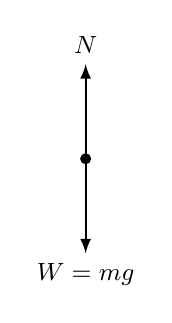
\begin{tikzpicture}[>=latex, font=\small]
  \fill (0,0) circle (2pt);
  \draw[->, thick] (0,0) -- (0,1.2) node[above] {$N$};
  \draw[->, thick] (0,0) -- (0,-1.2) node[below] {$W = mg$};
\end{tikzpicture}
\end{center}
\end{ejemplo}

\begin{aplicacion}[El cinturón de seguridad]
Cuando un bus frena de golpe, nadie te empuja hacia adelante: tu cuerpo simplemente sigue con
la velocidad que llevaba, porque sobre él no actúa la fuerza de frenado que sí actúa sobre el
bus. El cinturón de seguridad es la fuerza que te hace frenar junto con el vehículo.
\end{aplicacion}

\begin{preguntas}
% Ejercicio: leyes-newton-10-044
\pregunta Una caja de $\num{20,0}$ kg descansa sobre una mesa. ¿Cuál es su peso y cuál la
fuerza normal que actúa sobre ella?
\espacio{2cm}
% Ejercicio: leyes-newton-10-051
\pregunta Una caja que pesa $\num{77,0}$ N descansa sobre una mesa. Una cuerda atada a la caja
sube verticalmente, pasa por una polea y en el otro extremo cuelga un peso de $\num{30,0}$ N.
Determina la fuerza que ejerce la mesa sobre la caja.
\espacio{2.5cm}
% Ejercicio: leyes-newton-10-053
\pregunta Una caja que pesa $\num{77,0}$ N descansa sobre una mesa. Una cuerda atada a la caja
sube verticalmente, pasa por una polea y en el otro extremo cuelga un peso de $\num{90,0}$ N.
Determina la fuerza que ejerce la mesa sobre la caja.
\espacio{2.5cm}
% Ejercicio: leyes-newton-10-057
\pregunta Dos cubetas de pintura de $\num{3,2}$ kg cada una cuelgan una debajo de la otra
mediante dos cuerdas ligeras (la cuerda de arriba sostiene la cubeta superior y de esta cuelga
la otra). Si están en reposo, ¿cuál es la tensión en cada cuerda?
\espacio{3cm}
% PENDIENTE: el banco no tiene un ejercicio verificado de «encuentra el error» sobre la primera ley.
\end{preguntas}

\begin{resumen}
\begin{itemize}
  \item Fuerza neta cero $\Leftrightarrow$ reposo o velocidad constante (equilibrio).
  \item Diagrama de cuerpo libre: solo las fuerzas que \emph{otros} cuerpos ejercen sobre el
        cuerpo estudiado.
  \item En equilibrio: $\sum F_x = 0$ y $\sum F_y = 0$.
  \item Un cuerpo con velocidad constante no necesita una fuerza neta «a favor».
\end{itemize}
\end{resumen}

% ---------------------------------------------------------------------
\tema{Segunda ley de Newton}\label{tema:segundaley}

\begin{hilo}
La segunda ley es el corazón de los \emph{Principia}: dice \emph{cuánto} cambia la velocidad
cuando la fuerza neta no es cero. Du Châtelet, en su comentario, la escribió con el lenguaje
del cálculo, más cercano al que usamos hoy.
\end{hilo}

\begin{teorema}[Segunda ley de Newton]
La aceleración de un cuerpo es directamente proporcional a la fuerza neta que actúa sobre él,
inversamente proporcional a su masa, y tiene la dirección de la fuerza neta:
\[
  \sum \vec F = m\,\vec a.
\]
Un newton es la fuerza que acelera \qty{1}{kg} a \qty{1}{m/s^2}: $\qty{1}{N} = \qty{1}{kg.m/s^2}$.
\end{teorema}

La \textbf{masa} mide la inercia (cuánto cuesta cambiar la velocidad de un cuerpo) y no cambia
de un lugar a otro; el \textbf{peso} es la fuerza con que un planeta atrae al cuerpo, $W = mg$,
y sí cambia: en la Luna pesamos cerca de la sexta parte. La \textbf{fricción cinética}, cuando
un cuerpo se desliza, vale aproximadamente $f_k = \mu_k N$.

\begin{ejemplo}[Jalar una caja con fricción]
Una caja de \qty{20}{kg} se jala con \qty{80}{N} horizontales; $\mu_k = 0{,}25$. La normal es
$N = mg = \qty{196}{N}$, la fricción $f_k = 0{,}25 \times 196 = \qty{49}{N}$ y la fuerza neta,
$80 - 49 = \qty{31}{N}$. Entonces $a = 31/20 = \qty{1,55}{m/s^2}$.
\end{ejemplo}

\begin{aplicacion}[Frenar un bus del MIO]
Un bus articulado cargado tiene muchas veces la masa de un carro particular. Para detenerlo en
el mismo tiempo, con la misma aceleración, sus frenos deben hacer una fuerza muchas veces
mayor ($F = ma$). Por eso los buses frenan antes y tienen carriles exclusivos: su masa hace
que cada cambio de velocidad exija fuerzas enormes.
\end{aplicacion}

\begin{preguntas}
% Ejercicio: leyes-newton-10-032
\pregunta ¿Qué fuerza se requiere para acelerar a un niño sobre un trineo (masa total 55 kg) a
$\num{1,4}\ \mathrm{m/s^2}$?
\espacio{2cm}
% Ejercicio: leyes-newton-10-033
\pregunta Una fuerza neta de 265 N acelera a una persona en bicicleta a
$\num{2,30}\ \mathrm{m/s^2}$. ¿Cuál es la masa de la persona con la bicicleta?
\espacio{2cm}
% Ejercicio: leyes-newton-10-040
\pregunta ¿Qué fuerza promedio se requiere para detener en $\num{8,0}$ s un automóvil de 950 kg
que viaja a 95 km/h?
\espacio{2.5cm}
% Ejercicio: leyes-newton-10-060
\pregunta Un niño en un trineo llega a la base de una colina a $\num{10,0}$ m/s y luego recorre
$\num{25,0}$ m por una superficie horizontal hasta detenerse. Si juntos tienen una masa de
$\num{60,0}$ kg, ¿cuál es la fuerza retardadora promedio en el tramo horizontal?
\espacio{3cm}
% Ejercicio: leyes-newton-10-062
\Needspace{11\baselineskip}
\pregunta Un bloque de masa $m = \num{7,0}$ kg está sobre un plano liso (sin fricción) inclinado
$\num{22,0}^\circ$ respecto a la horizontal. Determina la aceleración del bloque al deslizarse
por el plano.
\espacio{3cm}
\end{preguntas}

\begin{resumen}
\begin{itemize}
  \item $\sum \vec F = m\,\vec a$: la aceleración tiene la dirección de la fuerza neta.
  \item Masa (kg) mide la inercia; peso (N) es $W = mg$.
  \item Fricción cinética: $f_k = \mu_k N$, opuesta al deslizamiento.
\end{itemize}
\end{resumen}

% ---------------------------------------------------------------------
\tema{Tercera ley de Newton}\label{tema:terceraley}

\begin{hilo}
La anécdota de la manzana tiene una segunda parte que Newton sí dejó escrita en su tercera ley:
si la Tierra atrae a la manzana, la manzana atrae a la Tierra con una fuerza igual.
\end{hilo}

\begin{teorema}[Tercera ley de Newton]
Si un cuerpo $A$ ejerce una fuerza sobre un cuerpo $B$, entonces $B$ ejerce sobre $A$ una
fuerza de igual magnitud y sentido contrario: $\vec F_{BA} = -\vec F_{AB}$.
\end{teorema}

Las dos fuerzas de un par acción--reacción actúan sobre cuerpos \emph{distintos}, por eso nunca
se anulan entre sí. Pueden ser de contacto (tus pies y el piso) o a distancia (la Tierra y la
Luna, dos imanes). Aunque las fuerzas sean iguales, los efectos pueden ser muy distintos,
porque cada cuerpo tiene su propia masa.

\begin{ejemplo}[La patinadora y la pared]
Una patinadora de \qty{50}{kg} empuja una pared con \qty{100}{N}. La pared la empuja a ella con
\qty{100}{N} en sentido contrario y, como casi no hay fricción con el hielo, sale hacia atrás
con $a = 100/50 = \qty{2}{m/s^2}$. La fuerza que ella ejerce actúa sobre la pared, no sobre
ella: por eso no «se cancela» con la otra~\cite{recurso10}.
\end{ejemplo}

\begin{aplicacion}[¿Qué empuja a un cohete?]
Un cohete no avanza porque sus gases empujen el suelo o el aire: el cohete empuja los gases
hacia abajo con gran fuerza, y los gases empujan el cohete hacia arriba con una fuerza igual.
Por eso un cohete funciona también en el vacío del espacio~\cite{recurso10}.
\end{aplicacion}

\begin{preguntas}
% Nuevos (el banco no tenía ningún ejercicio verificado de la tercera ley); ver el plan.
% Ejercicio: fuerzas-10-001
\Needspace{8\baselineskip}
\pregunta Un adulto de \qty{70}{kg} está parado sobre hielo (sin fricción) y un niño de
\qty{35}{kg}, bien apoyado en el piso, tira de una cuerda atada al adulto con una fuerza de
\qty{140}{N}. ¿Qué fuerza ejerce el adulto sobre el niño a través de la cuerda? ¿Qué
aceleración adquiere el adulto? ¿Por qué el niño no se mueve?
\espacio{3.5cm}
% Ejercicio: fuerzas-10-002
\pregunta Una manzana de \qty{0,20}{kg} cae de un árbol. La Tierra la atrae con su peso; por la
tercera ley, la manzana atrae a la Tierra con una fuerza igual. Calcula esa fuerza y la
aceleración que produce en la Tierra ($M_T = \qty{5,97e24}{kg}$). ¿Por qué no notamos que la
Tierra «sube» hacia la manzana?
\espacio{3.5cm}
% Pendiente de aprobación de la docente (manual-pendiente), no se incluye todavía:
% Ejercicio: leyes-newton-10-025 (juego de halar la cuerda y la tercera ley)
\end{preguntas}

\begin{resumen}
\begin{itemize}
  \item Acción y reacción: igual magnitud, sentidos contrarios, sobre cuerpos distintos.
  \item Existen pares de contacto y a distancia.
  \item Fuerzas iguales pueden producir aceleraciones muy distintas ($a = F/m$).
\end{itemize}
\end{resumen}

% ---------------------------------------------------------------------
\tema{Las tres leyes juntas}\label{tema:tresleyes}

\begin{hilo}
Los \emph{Principia} no se quedan en las leyes: las usan, una y otra vez, para resolver
problemas. Es lo que haremos al cerrar el trimestre.
\end{hilo}

Para resolver un problema de dinámica: (1) elige el cuerpo o el sistema; (2) dibuja su
diagrama de cuerpo libre; (3) elige ejes, uno en la dirección de la aceleración si la hay;
(4) escribe $\sum F_x = m a_x$ y $\sum F_y = m a_y$; (5) usa la tercera ley para relacionar
las fuerzas entre cuerpos que interactúan y la cinemática para traducir aceleraciones en
velocidades y distancias; (6) revisa unidades y orden de magnitud.

\begin{aplicacion}[El ascensor]
En un ascensor que arranca hacia arriba te sientes más pesado: el piso tiene que empujarte con
una normal mayor que tu peso para acelerarte ($N - mg = ma$). Cuando arranca hacia abajo, la
normal es menor y te sientes más liviano. Una báscula dentro del ascensor mide esa normal.
\end{aplicacion}

\begin{preguntas}
% Ejercicio: leyes-newton-10-058
\Needspace{7\baselineskip}
\pregunta Las dos cubetas de $\num{3,2}$ kg se jalan hacia arriba por la cuerda superior con una
aceleración de $\num{1,25}\ \mathrm{m/s^2}$. Calcula la tensión en cada cuerda.
\espacio{3cm}
% Ejercicio: leyes-newton-10-061
\pregunta Un adolescente en patineta, con rapidez inicial de $\num{2,0}$ m/s, baja rodando casi
sin fricción por un plano inclinado recto de 18 m de largo en $\num{3,3}$ s. ¿Cuál es el
ángulo de inclinación $\theta$ del plano?
\espacio{3.5cm}
% Ejercicio: leyes-newton-10-064
\pregunta A un bloque se le da una rapidez inicial de $\num{4,5}$ m/s hacia arriba de un plano
liso inclinado $22^\circ$. ¿Qué distancia sube por el plano?
\espacio{3cm}
\end{preguntas}

\begin{resumen}
\begin{itemize}
  \item Primero el diagrama de cuerpo libre; después las ecuaciones por componentes.
  \item La segunda ley da la aceleración; la cinemática, las velocidades y distancias.
  \item La tercera ley conecta las fuerzas entre cuerpos que interactúan.
\end{itemize}
\end{resumen}

% ---------------------------------------------------------------------
% 5. Saber 11
% ---------------------------------------------------------------------
\seccion{Prepárate para Saber 11}

\begin{preguntas}
% PENDIENTE: el banco no tiene preguntas tipo Saber verificadas de leyes de Newton.
% Ejercicio: cinematica-10-002
\pregunta Un automóvil viaja a una rapidez constante de 50 km/h durante 100 km. Luego acelera a
100 km/h y recorre otros 100 km. ¿Cuál es la rapidez promedio de su viaje de 200 km?
\begin{opciones*}(4)
  \item 67 km/h
  \item 75 km/h
  \item 81 km/h
  \item 50 km/h
\end{opciones*}

% Ejercicio: mediciones-10-071
\pregunta Tres estudiantes obtienen las siguientes ecuaciones, donde $x$ es la distancia
recorrida, $v$ la rapidez, $a$ la aceleración, $t$ el tiempo y el subíndice 0 indica el valor
en $t = 0$. ¿Cuál es correcta según una comprobación dimensional?
\begin{opciones*}(3)
  \item $x = vt^{2} + 2at$
  \item $x = v_{0}t + \frac{1}{2}at^{2}$
  \item $x = v_{0}t + 2at^{2}$
\end{opciones*}

% Ejercicio: cinematica-10-008
\Needspace{5\baselineskip}
\pregunta Un automóvil parte del reposo y acelera a $10\ \mathrm{m/s^2}$ constantes durante una
carrera de un cuarto de milla (402 m). ¿Qué tan rápido viaja cuando cruza la línea de meta?
\begin{opciones*}(4)
  \item 8090 m/s
  \item 90 m/s
  \item 81 m/s
  \item 809 m/s
\end{opciones*}
\end{preguntas}

% ---------------------------------------------------------------------
% 6. Cierre del hilo conductor
% ---------------------------------------------------------------------
\seccion{Cierre: de un plano inclinado a los \emph{Principia}}

Empezamos con Galileo imaginando un plano sin roce y terminamos con tres leyes que explican
por qué frena un bus, cómo sube un ascensor y qué empuja a un cohete. Newton se reconoció
«de pie sobre hombros de gigantes»; Halley hizo posible que su libro existiera; y Émilie du
Châtelet lo volvió legible para quienes vinieron después. Ahora tú también puedes usar esas
leyes.

Pero los \emph{Principia} no terminan en la tercera ley. Su libro tercero usa las mismas leyes
para explicar el movimiento de la Luna y de los planetas con una sola fuerza: la gravitación
universal. En el trimestre II aplicaremos la dinámica al movimiento en dos dimensiones
---proyectiles y movimiento circular--- y llegaremos a la gravitación.

% ---------------------------------------------------------------------
% 7. Evaluación
% ---------------------------------------------------------------------
\matrizevaluacion
  {Enuncia las tres leyes de Newton y reconoce cuándo un cuerpo está en equilibrio.}
  {Dibuja diagramas de cuerpo libre, suma fuerzas por componentes y calcula aceleraciones con unidades del SI y cifras adecuadas.}
  {Distingue los hechos documentados de las anécdotas y leyendas, y revisa si sus resultados son razonables.}
  {Trabaja en equipo en los laboratorios y comparte sus datos con honestidad.}

\autoevaluacion

\seguimientodocente

% ---------------------------------------------------------------------
% 8. Referencias
% ---------------------------------------------------------------------
\begin{referencias}
% verificado: https://www.bipm.org/en/-/2021-kg-consensus — BIPM: la nueva definición del kilogramo, basada en el valor fijo de la constante de Planck, entró en vigor el 20 de mayo de 2019
\bibitem{bipm} Bureau International des Poids et Mesures (BIPM). \emph{Kilogram: consensus
  value and dissemination}. Consultado el 14 de septiembre de 2026.
% verificado: https://www.e-rara.ch/doi/10.3931/e-rara-14635 — pie de imprenta: Desaint & Saillant; Lambert, 2 vols., 1756–1759
\bibitem{chatelet1759} Du Châtelet, É. (1759). \emph{Principes mathématiques de la
  philosophie naturelle} (2 vols., 1756--1759). París: Desaint \& Saillant; Lambert.
% verificado: https://portalegalileo.museogalileo.it/igjr.asp?c=36308 — Museo Galileo: Discorsi, Leiden, Elzevir, 1638 (plano inclinado y reloj de agua: https://galileo.library.rice.edu/lib/student_work/experiment95/inclined_plane.html)
\bibitem{galileo1638} Galilei, G. (1638). \emph{Discorsi e dimostrazioni matematiche intorno
  a due nuove scienze}. Leiden: Elzevir.
% verificado: recursos/fisica/Guías pedagógicas Física/markdown/10 - Guia_de_apoyo_cinematica_y_dinamica_grado_10_fisica.md (archivo local), caps. 1–4
\bibitem{recurso10} Guía de apoyo de Física 10.º: \emph{Cinemática y dinámica}, caps. 1--4.
  Material del colegio.
% verificado: https://mathshistory.st-andrews.ac.uk/Biographies/Halley/ — Halley animó a Newton a escribir los Principia, pagó la edición porque la Royal Society no tenía fondos y corrigió las pruebas
\bibitem{halley} MacTutor History of Mathematics. \emph{Edmond Halley}. University of St
  Andrews. Consultado el 14 de septiembre de 2026.
% verificado: https://www.colombiaaprende.edu.co/sites/default/files/files_public/2022-06/DBA_C.Naturales-min.pdf — PDF oficial del MEN publicado en Colombia Aprende
\bibitem{mendba} Ministerio de Educación Nacional (2016). \emph{Derechos Básicos de
  Aprendizaje V.1: Ciencias Naturales}. Bogotá: MEN.
% verificado: https://archive.org/details/McGillLibrary-osl_newton-philosophiae-naturalis-principia-mathematica_N563p1687-20098 — facsímil de la 1.ª ed., Londres, 1687 (imprimatur de Pepys y Historia piscium: https://royalsociety.org/blog/2014/07/principia/)
\bibitem{newton1687} Newton, I. (1687). \emph{Philosophiæ naturalis principia mathematica}.
  Londres: Joseph Streater, para la Royal Society.
% verificado: https://www.thelatinlibrary.com/newton.leges.html — Axiomata sive leges motus, 3.ª ed. (Londres, 1726)
\bibitem{newton1726} Newton, I. (1726). \emph{Philosophiæ naturalis principia mathematica}
  (3.ª ed.). Londres: Innys. «Axiomata, sive leges motus».
% verificado: https://physicsworld.com/a/the-legend-of-the-leaning-tower/ — Viviani es la única fuente de la historia de la torre; la mayoría de los historiadores dudan (1654: https://upittpress.org/wp-content/uploads/2018/07/9780822944072exr.pdf)
\bibitem{physicsworld} Physics World. \emph{The legend of the leaning tower}. Consultado el 14
  de septiembre de 2026.
% verificado: https://plato.stanford.edu/entries/emilie-du-chatelet/ — 1706–1749; Institutions de physique (1740); traducción de los Principia terminada en 1749 y publicada en 1759; «still the leading French translation»
\bibitem{sepChatelet} Stanford Encyclopedia of Philosophy. \emph{Émilie du Châtelet}.
  Consultado el 14 de septiembre de 2026.
% verificado: https://newtonproject.ox.ac.uk/view/texts/normalized/OTHE00001 — Stukeley, Revised Memoir of Newton (1752), Royal Society MS/142; conversación del 15 de abril de 1726
\bibitem{stukeley} Stukeley, W. (1752). \emph{Memoirs of Sir Isaac Newton's life}
  [manuscrito]. Royal Society, MS/142.
\end{referencias}

\end{document}
